% This file was created by matlab2tikz v0.4.3.
% Copyright (c) 2008--2013, Nico Schlömer <nico.schloemer@gmail.com>
% All rights reserved.
% 
\tikzsetnextfilename{plots/complexBot_eps}
%
% defining custom colors
\definecolor{mycolor1}{rgb}{0,0,0.5625}%
%
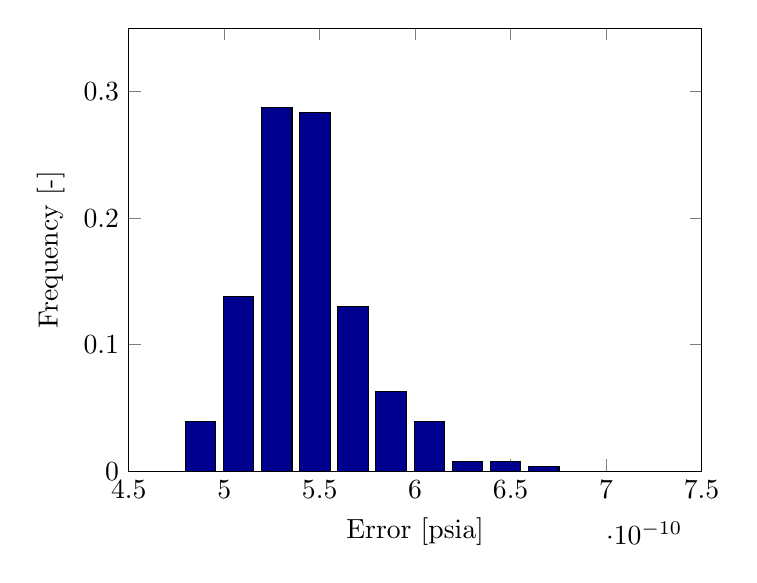
\begin{tikzpicture}

\begin{axis}[%
width=0.6\textwidth,
height=0.464012560662289\textwidth,
area legend,
scale only axis,
xmin=4.5e-10,
xmax=7.5e-10,
xlabel={Error [psia]},
ymin=0,
ymax=0.35,
ylabel={Frequency [-]}
]
\addplot[ybar,bar width=0.0319596438203007\textwidth,draw=black,fill=mycolor1] plot coordinates{(4.87585793962353e-10,0.0393700787401575)
(5.07560571350041e-10,0.137795275590551)
(5.27535348737729e-10,0.28740157480315)
(5.47510126125417e-10,0.283464566929134)
(5.67484903513105e-10,0.12992125984252)
(5.87459680900793e-10,0.062992125984252)
(6.07434458288481e-10,0.0393700787401575)
(6.27409235676168e-10,0.0078740157480315)
(6.47384013063856e-10,0.0078740157480315)
(6.67358790451544e-10,0.00393700787401575)};

\addplot [
color=black,
solid,
forget plot
]
table[row sep=crcr]{
4.5e-10 0\\
7.5e-10 0\\
};
\end{axis}
\end{tikzpicture}%